\section{Loop Transformer 的核心机制：把迭代放回隐藏状态}
\label{sec:loop-transformer-core}

本章的中心判断是：Loop Transformer 把 CoT 的外部文本循环压缩为隐藏状态递归。它复用少量 Transformer 层组成共享模块，让前一次循环得到的隐藏状态成为下一次循环的输入。这样做的收益是参数更紧凑、计算过程更贴近连续表示；风险是同一模块被反复应用后，稳定性、表达能力和训练监督都会变成新问题。

\begin{importantbox}{本章主张}
Loop Transformer 的核心机制可以概括为一句话：同一个共享 Transformer 模块 \(F_\theta\) 多次作用于隐藏状态 \(h_t\)，用递归深度换取有效计算深度。
\end{importantbox}

\subsection{从 CoT 管线到隐藏状态循环}

上一章已经说明，CoT 的中间步骤要经历解码、文本追加、重新分词、重新嵌入。若把模型内部表示想成“工作记忆”，CoT 像把工作记忆的一部分写到纸上，再把纸上的文字重新读进脑中。这个类比有用，因为它点出了成本来源：真正需要更新的是隐藏表示，实际通道却绕了一圈文本。

Loop Transformer 的直觉是直接更新工作记忆。模型不必把每个中间想法先写成 token；它可以把当前隐藏状态留在连续向量空间中，并让同一个模块继续修改这份状态。视频中的“looping hidden states”画面正是在强调这个转换：推理循环从外部文本轨迹转入内部状态轨迹。

\begin{figure}[htbp]
    \centering
    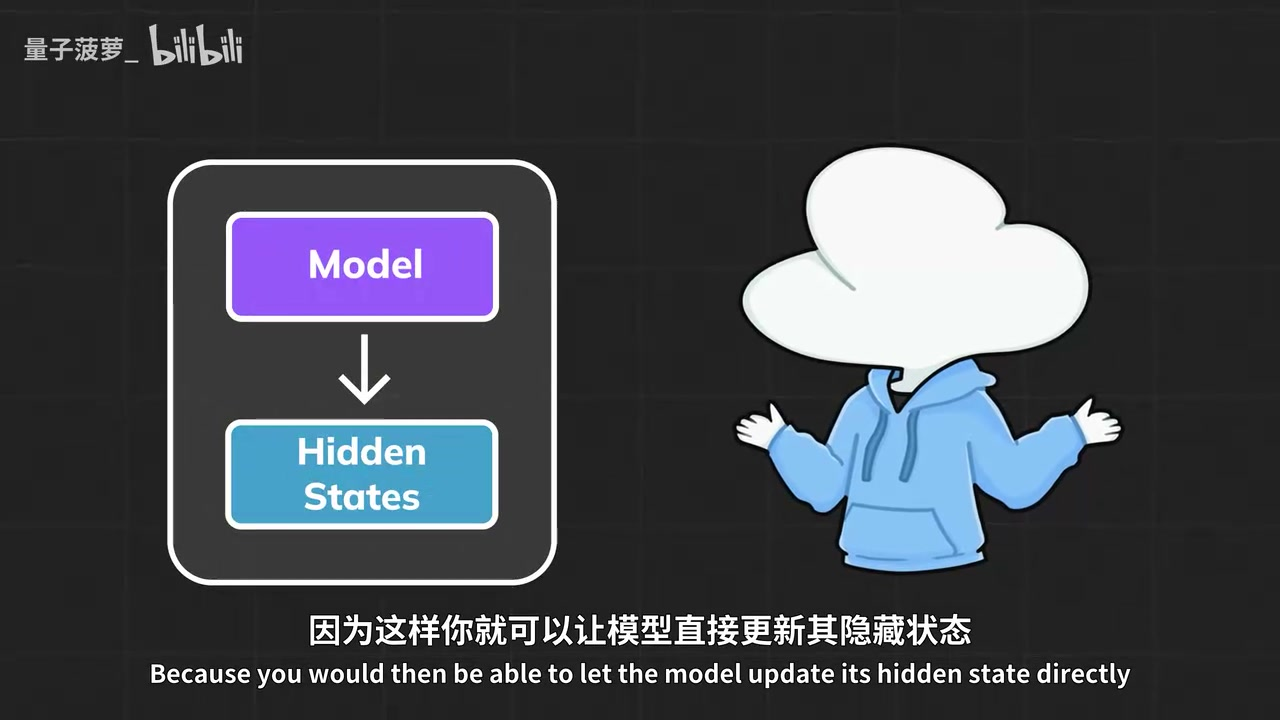
\includegraphics[width=0.82\linewidth,height=0.34\textheight,keepaspectratio]{figures/fig_04_looping_hidden_states.jpg}
    \caption{隐藏状态循环：Loop Transformer 让模型直接更新内部表示，把推理迭代放入连续状态空间。\protect\footnotemark}
    \label{fig:loop-hidden-state-update}
\end{figure}
\footnotetext{视频画面时间区间：00:04:52--00:05:04。}

\begin{knowledgebox}{类比的边界}
“脑内打磨草稿”只是帮助理解的类比。技术上，隐藏状态是高维连续向量；每次递归更新都会经过注意力、前馈网络、残差连接和归一化等操作。类比解释动机，公式和结构解释机制。
\end{knowledgebox}

\subsection{基本递归公式：同一模块反复更新状态}

先用普通话说明公式含义：循环 Transformer 把当前隐藏状态当成可更新的状态变量，把输入 \(x\) 当成问题和上下文条件，再把同一个带参数模块 \(F_\theta\) 应用到当前状态上，得到下一轮隐藏状态。多跑一次循环，就多做一次内部表示更新。

$$
h_{t+1}=F_\theta(h_t,x)
$$

符号说明如下：
\begin{itemize}
    \item \(h_t\)：第 \(t\) 次递归后的隐藏状态，承载模型当前的内部表示。
    \item \(h_{t+1}\)：下一次递归后的隐藏状态，也就是一次内部更新之后的新工作记忆。
    \item \(x\)：输入 token、位置、上下文或注入到循环模块中的条件信息。
    \item \(F_\theta\)：共享的 Transformer 递归模块，可以包含注意力层、前馈层和归一化结构。
    \item \(\theta\)：模块参数，在不同递归步之间共享。
    \item \(t\)：递归步编号，表示模型已经在内部循环了多少轮。
\end{itemize}

这个公式的重点在“共享”。标准深层 Transformer 可以把第 1 层、第 2 层、第 3 层分别看成不同函数；Loop Transformer 让同一个函数多次处理不断变化的状态。直观地说，参数量没有按深度线性增长，有效计算步数却可以随递归次数增长。

\subsection{残差更新：让新信息叠加到旧状态上}

实际 Transformer 中，信息通常沿残差流（residual stream）累积。残差形式的直觉是：当前状态 \(h_t\) 先保留下来，模块 \(F_\theta\) 计算一个更新量，再把旧状态和更新量相加，最后用归一化控制数值尺度。这样写可以更接近 Transformer 的信息流，也为后文稳定性章节铺路。

$$
h_{t+1}=\mathrm{Norm}\bigl(h_t+F_\theta(h_t,x)\bigr)
$$

符号说明如下：
\begin{itemize}
    \item \(h_t\)：进入本轮递归前的残差流状态。
    \item \(F_\theta(h_t,x)\)：共享模块根据当前状态和输入条件产生的更新量。
    \item \(h_t+F_\theta(h_t,x)\)：把旧状态与新更新叠加后的临时状态。
    \item \(\mathrm{Norm}(\cdot)\)：归一化操作，用于控制尺度并降低状态范数失控的风险。
    \item \(h_{t+1}\)：归一化之后传给下一轮递归的状态。
\end{itemize}

这条公式解释了 Loop Transformer 与普通“重复跑同一层”的区别。模型每轮沿着已有状态继续计算，并在同一条残差流上持续改写表示。状态保留了前面递归的结果，更新量则把新注意到的关系、事实或约束叠加进去。

\subsection{共享 Transformer 块：用递归深度形成有效深度}

视频中展示的 recurrent Transformer block 把机制画得更具体：一个包含多头注意力（Multi-Head Attention）和前馈网络（Feed-Forward）的块被环形箭头包住，表示输出会回到同一块中继续处理。前一次循环的输出隐藏状态成为下一次循环的输入，这正是“循环”一词的结构含义。

\begin{figure}[htbp]
    \centering
    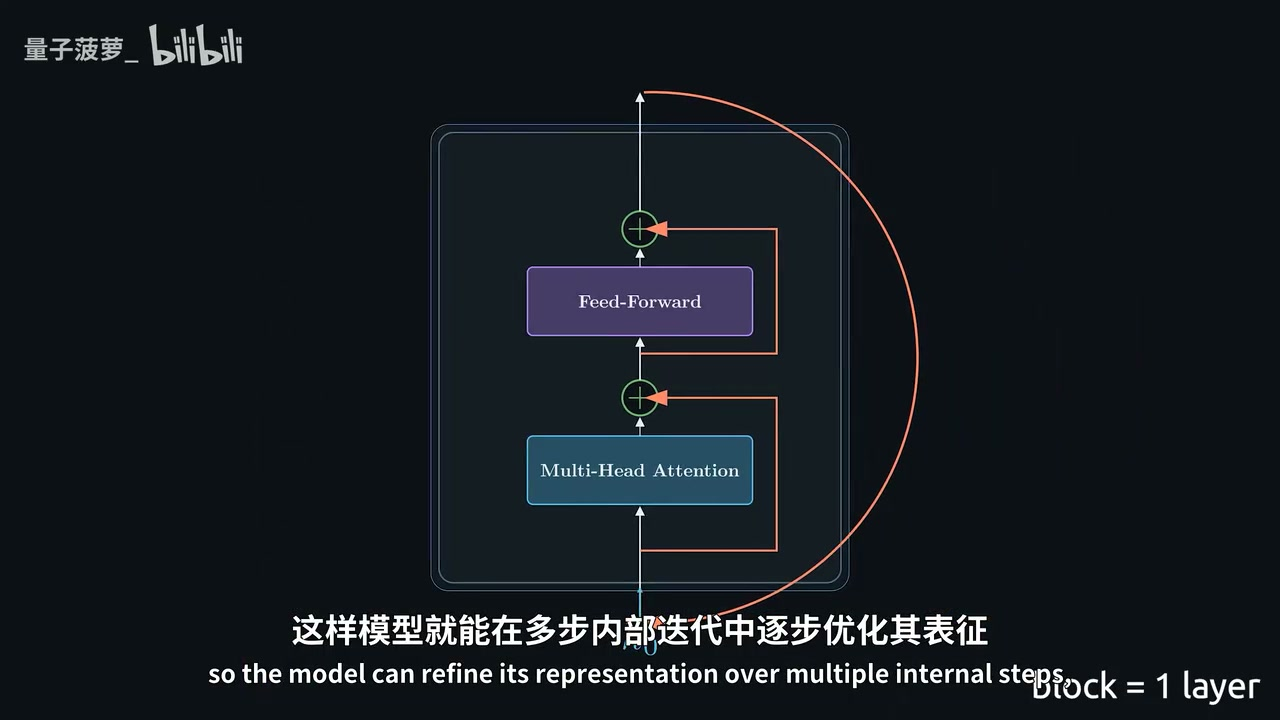
\includegraphics[width=0.82\linewidth,height=0.36\textheight,keepaspectratio]{figures/fig_05_recurrent_transformer_block.jpg}
    \caption{共享 Transformer 块反复作用于残差流，让模型在多步内部递归中逐步打磨表示。\protect\footnotemark}
    \label{fig:recurrent-transformer-block}
\end{figure}
\footnotetext{视频画面时间区间：00:05:25--00:05:40。}

这里有一个容易被忽略的点：共享权重并不自动意味着每一步功能相同。原因在于输入状态已经改变。同一个函数 \(F_\theta\) 处理 \(h_0\)、\(h_1\)、\(h_2\) 时，看到的是不同状态，因此可以表现出阶段化行为：早期整理问题，中期整合关系，后期收敛答案。第三章会把这个判断和行为证据连起来。

\begin{warningbox}{机制边界}
Loop Transformer 的“有效深度”来自重复应用共享模块。它能节省参数，也能提供更多内部更新机会；它同样带来约束，因为每一步都受同一组参数控制。后续章节需要继续检查：这种约束是否稳定、是否可外推、是否真的形成可复用推理过程。
\end{warningbox}

\subsection{本章小结}

本章把 Loop Transformer 的核心机制压缩成两条公式和一个结构图。基本公式 \(h_{t+1}=F_\theta(h_t,x)\) 表示同一共享模块递归更新隐藏状态；残差公式 \(h_{t+1}=\mathrm{Norm}(h_t+F_\theta(h_t,x))\) 表示更新沿残差流叠加并受归一化控制。这个设计把 CoT 的外部 token 循环转入内部状态循环，用递归深度换取有效计算深度。下一章要回答更关键的问题：这种内部递归是否带来了可观察的行为收益。
